\chapter{Lagrangian Domain: Vortex Particle Method}
\label{ch:theory}

%To model the flow around a VAWT, several approaches can be taken, Vermeer at al. (2003) \cite{Vermeer2003} have also summarized in their paper. The two main approaches of investigating the flow is either employing a numerical method to simulate the flow or through experimental simulations.

%Leishman (2006) \cite{leishman2006principles} has shown that there are several simplified, efficient numerical tools that can be used to model the performance of a VAWT. Methods such as actuator disk theory and blade element momentum theory and deals with simplified Navier-Stokes equations and is very useful to evaluate the trend of certain design parameter. However, as they are highly simplified, complex flow phenomenons that has severe impact of the performance characteristics of the VAWT such as flow separation during dynamic stall, vortex shedding during the rotation and blade-wake interaction cannot be simulated. In order to understand them, either experimental investigation such as in wind tunnel or full Navier-Stokes simulations have to undertaken. So to understand the flow behaviour of a VAWT, several numerical research have been performed \cite{Almohammadi2013} \cite{Ferreira2007} \cite{Islam2008} \cite{Merz2012} and experimental researches by Ferreira \cite{SimaoFerreira2008} \cite{Ferreira} and others \cite{Howell2010} \cite{Mertens2003}.
%\index{Actuator disk}

%All the numerical method that was grid-based struggled with dealing with large number of mesh cells for high Reynolds numbers and the numerical method that employed simplified Navier-Stokes methods had to sacrifices some accuracies.The experimental investigation also come with drawbacks as they are require more financial resources and usually only feasible to model the scaled VAWTs.

%This is the main relevance of the hybrid vortex particle method for the VAWT investigations. By utilizing the two methods together, the vortex particle method away from body, and Navier-Stokes solver with turbulence model in the near-body region, one will be able to tackle the challenges in an efficient manner.

%Therefore, this chapter is dedicated to given an overview on the theory of the Vortex Particle Method which we will employ with coupled Navier-Stokes solver. 


%------------------------------------------------------------------------------------------------------
%------------------------------------------------------------------------------------------------------
%------------------------------------------------------------------------------------------------------
\section{Introduction to Vortex Method}
\printAcron{Vortex Method}{VM} is a branch of computational fluid dynamics that deals with the evolution of the vorticity of the fluid in a lagrangian description. Typically, the fluid is viewed at a fixed window where it is described as a function of space \lsymb[t]{$\mathbf{x}$}{Position vector}{$[m]$}{x} and time \lsymb[t]{$t$}{Time}{$[s]$}{t}. However, the lagrangian point of view regards the fluid as a collection of the particles carrying the proprety of the fluid. 

\todo{Lagrangian vs. Eulerian fluid diagram}

Unlike the typical eulerian method that require discretization of all the fluid domain, vortex methods only needs fluid elements where there is vorticity. This means that the vortex method are inherently auto-adaptive method that only simulated the flow of interest. Furthermore, with the computational acceleration methods such as \printAcron{Fast-Multipole Method}{FMM} and parallel computation on \printAcron{Graphics Processing Units}{GPU}, vortex method can be more efficient that typical eulerian methods.

\subsection{Vorticity}
Vorticity \gsymb[t]{$\omega$}{Vorticity field}{$[1/s]$}{xx}, the governing element of vortex method, is defined as

\begin{equation}
\mathbf{\omega} = \Delta \times \mathbf{u},
\end{equation}

where \lsymb[t]{$\mathbf{u}$}{Velocity field}{$[ms^{-1}]$}{u} is the velocity field. The circulation \gsymb[t]{$\Gamma$}{Circulation}{$m^2s^{-1}$}{g} is defined as

\begin{equation}
\Gamma = \int_L\mathbf{u}\cdot d \mathbf{r}=\int_S\omega\cdot\mathbf{n}\ dS,
\end{equation}

by the stokes theorem, as represents the integral vorticity of the domain, figure \ref{fig:vorticityCirculation}

\begin{figure}[h]
\centering
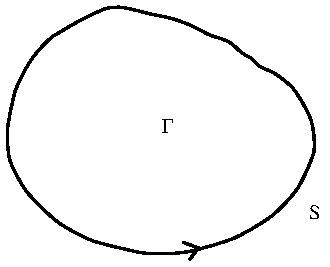
\includegraphics[width=0.2\linewidth]{./figures/lagrangian/vorticityCirculation.pdf}
\caption{Circulation of the fluid}
\label{fig:vorticityCirculation}
\end{figure}

 
\subsection{Velocity-vorticity formulation of navier-stokes equations}
The governing equation of the vortex method is velocity-vorticity $\mathbf{u}-\omega$ formulation of the navier-stokes equations \cite{Cottet2000a}. The 2-D incompressible navier-stokes momentum equation is given as

\begin{equation}
\frac{\partial \mathbf{u}}{\partial t} + \mathbf{u}\cdot\nabla\mathbf{u} = - \frac{1}{\rho} \nabla p + \nu \nabla^2\mathbf{u},
\label{eq:mom}
\end{equation}

relating the velocity field $\mathbf{u}\left(\mathbf{x},t\right)$ to the pressure field $\mathbf{p\left(\mathbf{x},t\right)}$ \lsymb[f]{$p$}{Pressure}{$[\mathbrm{Pa}]$}{p}, the kinematic viscosity \gsymb[t]{$\nu$}{Kinematic viscosity}{$[m^2/s]$}{mm} and density \gsymb[t]{$\rho$}{Density}{$[kg/m^3]$}{qq}. Furthermore, we also have to satisfy the incompressibility constraint given as

\begin{equation}
\nabla\cdot\mathbf{u} = 0.
\end{equation}

To attain the velocity-vorticity formulation, we should take the curl of the velocity-pressure $\mathbf{u}-p$ formulation of the navier-stokes equation. Taking the curl of the momentum equation \ref{eq:mom}, we get the vorticity transport equation

\begin{equation}
\frac{\partial \omega}{\partial t} + \mathbf{u}\cdot\nabla\omega = \nu \nabla^2 \omega,
\end{equation}

which only relates the vorticity to the velocity enabling us to neglect the pressure field.


\subsection{Viscous splitting algorithm}
Vortex method is initiality used to model the evolution of incompressible, invcid flows. However, in order to simulate a real flow, we must also deal with the viscous component of the fluid. Chorin \cite{Chorin1973} has shown that using the viscous spilliting algorithm, it is possible to model a viscous flow using vortex method. 

The viscous splitting algorithm is a fractional step method, where the viscous and the inviscid part of the transport equation is dealth in two subsquent steps, 

\begin{itemize}
\item convection:
\begin{equation}
\frac{\partial\omega}{\partial t} + \mathbf{u}\cdot\nabla\omega=0;
\label{eq:convectionEulerian}
\end{equation}
\item diffusion:
\begin{equation}
\frac{\partial\omega}{\partial t} = \nu\nabla^2\omega.
\end{equation}

\end{itemize}

Therefore, the evolution of the vorticity is split into two sub-steps. The first substep of the evolution deals with the convection of the vorticity and the second deals with the diffusion of the vorticity field. There are several ways of dealing with the diffusion of the vorticity field and Chorin initially employed a random walk method. This method suffers some limitations in accuracy and since then there are several methods that can be used to simulate the diffusion such as the \printAcron{Particle Strength Exchange}{PSE} method, redistribution method and core spreading method. 

%This equation is known as the vorticity transport equation \cite{LEONARD1995}. To solve this equation, we employ a viscous splitting algorithm, where the evolution of the vorticity field is convection and the diffusion of the vorticity field is handled i

%There are several advantage to this type of evolution. As the convection and diffusion are handled separately, there is minimum dispertion during the convection and furthermore, the is no restriction of the advection CFL number \cite{Wee2006}.


%------------------------------------------------------------------------------------------------------
%------------------------------------------------------------------------------------------------------
%------------------------------------------------------------------------------------------------------
\section{Spatial Discretization: Generation of Vortex Blobs}

Vortex blobs were first introduced by Chorin.

\subsection{Discrete form of vorticity field}
The spatial discretization of the fluid domain is done by representing the vorticity field in $N$ Lagrangian vortex particles. This is done by dividing the fluid domains into cells where the circulation of the region is assigned to the particle. This gives 

\begin{equation}
\omega\left(\mathbf{x},t\right) \simeq \omega^h\left(\mathbf{x},t\right) = \sum_{p}\Gamma_p\left(t\right)\zeta_{\sigma}\left[\mathbf{x}-\mathbf{x}_p\left(t\right)\right],
\end{equation}

\subsection{Mollified vortex kernels}

where $\Gamma_p$ \gsymb[f]{$\Gamma$}{Circulation}{$[m^2/s]$}{c} is the estimate of the circulation around the particle $\mathbf{x}_p$ \lsymb[f]{$\mathbf{x}_p$}{Position vector}{[-]}{x} with core size \gsymb[t]{$\sigma$}{Core size}{[$m$]}{rr}. We must not that $\omega^h$ is an approximation to $\omega$ of the fluid.

Due to the non-zero size of the vortex elemnts, it is refered to as vortex blobs. The advantage of the vortex blobs is that the with a smooth distribution of the vorticity, the singularity disappears and so numerical instability does not happen when blobs get too close to each other. 

An ideal choice for a cutoff function is a Gaussian distribution. Gaussian kernels satisfy the requirement for smooth distributon ad decays quickly. The Gaussian kernel is defined as

\begin{equation}
\zeta_{\sigma} = \frac{1}{k\pi\sigma^2}\exp\left(\frac{-\left|\mathbf{x}\right|}{k\sigma^2}\right),
\end{equation}

where $k$ is 1, 2 or 4 and determines the width of the kernel.

\begin{figure}
	\centering
	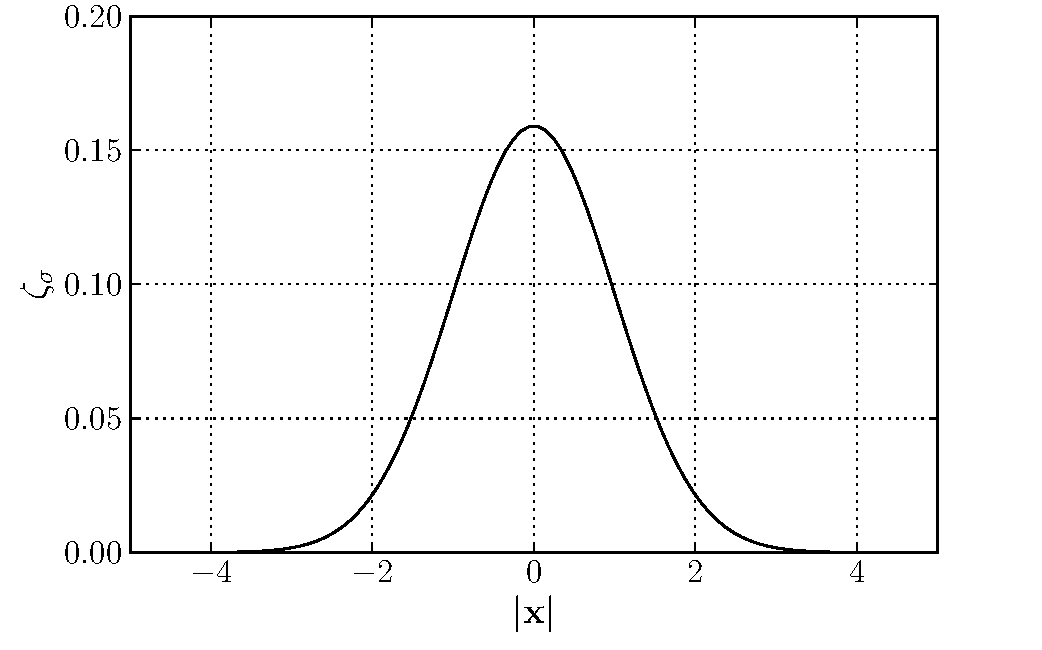
\includegraphics[width=0.7\textwidth]{figures/lagrangian/gaussianKernel.pdf}
	\caption{Vortex blob with Gaussian distribution: [$k=2$,$\sigma=1.0$]}
\end{figure}


\subsection{Beale's correction: Iterative circulation processing scheme}


\subsection{Error in blob initialization}

%------------------------------------------------------------------------------------------------------
%------------------------------------------------------------------------------------------------------
%------------------------------------------------------------------------------------------------------
\section{Convection of vortex blobs}


\subsection{Biot-savart law}
The vortex transport equation evaluated using the viscous splitting algorithm. For vortex methods, it is ideal to express the equation \ref{eq:convectionEulerian} in Lagrangian form,

\begin{equation}
\frac{\mathrm{d}\mathbf{x}_p}{\mathrm{d}t} = \mathbf{u}\left(\mathbf{x}_p\right),
\end{equation}
with
\begin{equation}
\frac{\mathrm{d}\omega_p}{\mathrm{d}t} = 0.
\end{equation}

The velocity field can be decomposed using the Helmoltz decomposition,
\begin{equation}
\mathbf{u} = \mathbf{u}_{\infty} + \mathbf{u}_{\omega}
\end{equation}
with \lsymb[t]{$\mathbf{u}_{\infty}$}{Free-stream velocity}{$[m/s]$}{ul} as the free-stream velocity, \lsymb[t]{$\mathbf{u}_{\omega}$}{Vortical velocity}{$[m/s]$}{uxx} as the velocity of the vortical part of the flow.


The velocity can be related to the vorticity using the Biot-Savart law
\begin{equation}
\mathbf{u} = \mathbf{u}_{\infty} + \mathbf{K}\star\omega,
\end{equation}
\begin{equation}
\mathbf{u} = \mathbf{u}_{\infty} + \mathbf{K}\star\omega,
\end{equation}

where the $\star$ represents convolution of the kernel $\mathbf{K}_p$ given by

\begin{equation}
\mathbf{K}_p = \frac{1}{2\pi\left|\mathbf{x}\right|^2}\left(-x_2,x_1\right).
\label{eq:GreensKernel}
\end{equation}

The advantage of discretizing and evaluting the vorticity field in this form is that vortex elements are only needed where the vorticity is nonzero. This means that the vortex elements inherently adapts to domain of interest and does not require simulation of region where nothing happens. From equation \ref{eq:GreensKernel}, we see that it has a singularity when the particles approach each other and so to overcome this we can mollify the kernel using a smooth cutoff function \gsymb[t]{$\zeta$}{Smooth cutoff function}{[-]}{ff}. So the mollified kernel $\mathbf{K}_{\epsilon}$ is given as 

\begin{equation}
\mathbf{K}_{\epsilon} = \mathbf{K} \star \zeta_{\epsilon}.
\end{equation}

\subsection{Remeshing scheme: Treating lagrangian grid distortion}

%------------------------------------------------------------------------------------------------------
%------------------------------------------------------------------------------------------------------
%------------------------------------------------------------------------------------------------------
\section{Diffusion of Vortex Methods}

\subsection{Vorticity diffusion techniques}

\subsection{Modified remeshing for treating diffusion}

%\subsection{Convergence of the viscous vortex method}
%------------------------------------------------------------------------------------------------------
%------------------------------------------------------------------------------------------------------
%------------------------------------------------------------------------------------------------------
\section{Boundary conditions at solid boundary}

\subsection{Boundary integral equations}

\subsubsection{Linked boundary conditions}

\subsection{Panel method for treating no-slip boundary condition}

\subsection{Convergence study of panel method}

\section{Simulation acceleration techniques}

\subsection{Fast multi-pole Method}

\subsection{Parallel computation in GPU}

\section{Validation of lagrangian method}

\subsection{Lamb-oseen vortex at $Re=100$}

\subsection{Convection of Clercx-Bruneau dipole at $Re=625$}

\section{Summary}



%\section{Convection step}
%
%The convection step of the vorticity transport equation is define by following equation
%
%\begin{equation}
%\frac{d\mathbf{x}_i}{dt} = \mathbf{u}_i\left(\mathbf{x}_1,\mathbf{x}_2,...,\mathbf{x}_N,t\right),
%\end{equation}
%
%and we have to ensure that the circulation is conserved,
%
%\begin{equation}
%\frac{d\Gamma}{dt} = 0.
%\end{equation}
